% SYS810 - Devoir 1.tex (Version 2.0)
% ===============================================================================
% ETS SYS810 Devoirs templates.
% Based on ANUfinalexam.tex 2004; 2009, Timothy Kam, ANU School of Economics
% Licence type: Free as defined in the GNU General Public Licence: http://www.gnu.org/licenses/gpl.html

\documentclass[a4paper,12pt,fleqn]{article}
\usepackage{amsmath}
\usepackage{empheq}
\usepackage{fancyhdr}
\usepackage{epigraph}
\usepackage{placeins}
\usepackage[]{mcode}

\usepackage[utf8]{inputenc} 

% Insert your course information here %%%%%%%%%%%%%%%%%%%%%%%%%%%%%%%%%%

\newcommand{\institution}{École de Technologie Supérieure}
\newcommand{\titlehd}{Simulation numérique des systèmes}
\newcommand{\examtype}{Devoir 1}
\newcommand{\examdate}{Février 2015}
\newcommand{\examcode}{SYS 810}
\newcommand{\authors}{Milan Assuied, Adam Burney}
\newcommand{\lastwords}{Fin du devoir}

% Insert recurent maths notations %%%%%%%%%%%%%%%%%%%%%%%%%%%%%%%%%%
\def\mean#1{\left< #1 \right>}

% Common commands
\newcommand{\Xzero}{x_0}
\newcommand{\Xone}{x_1}
\newcommand{\Xtwo}{x_2}

% Commands for exercice one
\newcommand{\Ir}{i_r}
\newcommand{\Ic}{i_c}
\newcommand{\Is}{i_2}
\newcommand{\Il}{i_l}
\newcommand{\DIl}{\frac{d\Il}{dt}}

\newcommand{\Vc}{e_c}
\newcommand{\Vi}{e_i}
\newcommand{\Vr}{e_r}
\newcommand{\Vl}{e_l}
\newcommand{\DVc}{\frac{d\Vc}{dt}}

\newcommand{\StateMatrix}{
\begin{bmatrix}
\Xone\\
\Xtwo\end{bmatrix}
=
\begin{bmatrix}
\Vc\\
\Il\end{bmatrix}}

\newcommand{\DXone}{\frac{d\Xone}{dt}}
\newcommand{\DXtwo}{\frac{d\Xtwo}{dt}}

\newcommand{\StateMatrixALineOne}{}
\newcommand{\StateMatrixALineTwo}{}
\newcommand{\StateMatrixBLineOne}{}
\newcommand{\StateMatrixBLineTwo}{}

% Commands for exercice two
\newcommand{\X}{x}
\newcommand{\Xl}{x_l}
\newcommand{\dX}{\frac{d\X}{dt}}
\newcommand{\ddX}{\frac{d^2\X}{dt^2}}

\newcommand{\M}{M}
\newcommand{\Kone}{k_1}
\newcommand{\Ktwo}{k_2}
\newcommand{\B}{b}
\newcommand{\XlLit}{\frac{\M.g}{\Kone}+\Xzero}

\newcommand{\Fm}{F_M}
\newcommand{\Fs}{F_s}
%%%%%%%%%%%%%%%%%%%%%%%%%%%%%%%%%%%%%%%%%%%%%%%%%%%%

%\setcounter{MaxMatrixCols}{10}
\newtheorem{theorem}{Theorem}
\newtheorem{acknowledgement}[theorem]{Acknowledgement}
\newtheorem{algorithm}[theorem]{Algorithm}
\newtheorem{axiom}[theorem]{Axiom}
\newtheorem{case}[theorem]{Case}
\newtheorem{claim}[theorem]{Claim}
\newtheorem{conclusion}[theorem]{Conclusion}
\newtheorem{condition}[theorem]{Condition}
\newtheorem{conjecture}[theorem]{Conjecture}
\newtheorem{corollary}[theorem]{Corollary}
\newtheorem{criterion}[theorem]{Criterion}
\newtheorem{definition}[theorem]{Definition}
\newtheorem{example}[theorem]{Example}
\newtheorem{exercise}[theorem]{Exercise}
\newtheorem{lemma}[theorem]{Lemma}
\newtheorem{notation}[theorem]{Notation}
\newtheorem{problem}[theorem]{Problem}
\newtheorem{proposition}[theorem]{Proposition}
\newtheorem{remark}[theorem]{Remark}
\newtheorem{solution}[theorem]{Solution}
\newtheorem{summary}[theorem]{Summary}
\newenvironment{proof}[1][Proof]{\noindent\textbf{#1.} }{\ \rule{0.5em}{0.5em}}

% ANU Exams Office mandated margins and footer style
\setlength{\topmargin}{0cm}
\setlength{\textheight}{9.25in}
\setlength{\oddsidemargin}{0.0in}
\setlength{\evensidemargin}{0.0in}
\setlength{\textwidth}{16cm}
\pagestyle{fancy}
\lhead{} 
\chead{} 
\rhead{} 
\lfoot{} 
\cfoot{\footnotesize{Page \thepage \ of \pageref{finalpage} -- \titlehd \ (\examcode)}} 
\rfoot{} 

\renewcommand{\headrulewidth}{0pt} %Do not print a rule below the header
\renewcommand{\footrulewidth}{0pt}


\begin{document}

% Title page

\begin{center}
%\vspace{5cm}
\large\textbf{\institution}
\end{center}
\vspace{1cm}

\begin{center}
\textit{ \examtype -- \examdate}
\end{center}
\vspace{1cm}

\begin{center}
\large\textbf{\titlehd}
\end{center}

\begin{center}
\large\textbf{\examcode}
\end{center}
\begin{center}
\large\textbf{\authors}
\end{center}https://www.sharelatex.com/project/
\vspace{4cm}

% End title page


\numberwithin{equation}{section}

% START OF EXERCICE 1 %
\newpage
\section{\textbf{Problème 1}}
Circuit électrique non linéaire
\begin{enumerate}
\item \underline{Écrire la représentation d'état non linéaire de ce circuit.}\\ \underline{Choisir comme variables d'état $x_1 = e_c$ et $x_2 = i_l$.}

Les équations du circuit s'écrivent:
\begin{align}
\Is + \Ic &= \Ir + \Il \label{eq:1} \\
\Vi &= \Vc + \Vl \label{eq:2} \\
&= \Vc + \Vr \label{eq:3} \\
\Vr &= \Vl \nonumber
\end{align}

De \eqref{eq:1}  il vient:
\begin{align} \label{eq:etat1}
&\frac{1}{8}\Vc^3+C\DVc = \Il + \Ir \nonumber \\
\intertext{or de \eqref{eq:3}:}
&\Ir = \frac{1}{R}\Vi - \frac{1}{R}\Vc  \nonumber \\
\intertext{Il en résulte:}
\Aboxed{&\DVc = -\frac{1}{8C}\Vc^3-\frac{1}{RC}\Vc+\frac{1}{C}\Il+\frac{1}{RC}\Vi}
\end{align}

De \eqref{eq:2} il vient:
\begin{align}\label{eq:etat2}
\Vi& = \Vc + \Vl \nonumber \\
\Vi& = \Vc + L\DIl \nonumber \\
\Aboxed{\DIl& = -\frac{1}{L}\Vc + \frac{1}{L}\Vi}
\end{align}

\renewcommand{\StateMatrixALineOne}{-\frac{1}{8C}\Xone^3-\frac{1}{RC}\Xone+\frac{1}{C}\Xtwo}
\renewcommand{\StateMatrixALineTwo}{-\frac{1}{L}\Xone}
\renewcommand{\StateMatrixBLineOne}{\frac{1}{RC}\cdot\Vi}
\renewcommand{\StateMatrixBLineTwo}{ \frac{1}{L}\cdot\Vi}

De \eqref{eq:etat1} et \eqref{eq:etat2} on déduit la représentation d'état:

 \begin{empheq}[left=\empheqlbrace, box=\fbox]{align}\label{eq:stateEquation}
    \DXone &= \StateMatrixALineOne + \StateMatrixBLineOne , & \StateMatrix \nonumber \\
    \DXtwo &= \StateMatrixALineTwo + \StateMatrixBLineTwo
\end{empheq}

\newpage
\item \underline{Déterminer le point d'équilibre du système.}

L'équilibre est donné par
\begin{empheq}[left=\empheqlbrace]{align*}
-\frac{1}{8C}\Vc^{*^3}-\frac{1}{RC}\Vc^{*}+\frac{1}{C}\Il^{*}+\frac{1}{RC}\mean{\Vi}& = 0\\
-\frac{1}{L}\Vc^{*} + \frac{1}{L}\mean{\Vi}& = 0 
\end{empheq}

Soit:
\begin{empheq}[left=\empheqlbrace]{align*}
-\frac{1}{8C}\mean{\Vi}^3-\frac{1}{RC}\mean{\Vi}+\frac{1}{C}\Il^{*}+\frac{1}{RC}\mean{\Vi}& = 0\\
\Vc^{*}& = \mean{\Vi}
\end{empheq}

Finalement:
\begin{empheq}[left=\empheqlbrace, box=\fbox]{align}
\Il^{*}& = \frac{1}{8}\mean{\Vi}^3 \nonumber\\ 
\Vc^{*}& = \mean{\Vi}
\end{empheq}

On linéarise autour du point d'équilibre:

\begin{equation*}
\dot{\delta}{x} = \left.\frac{\partial{F}}{\partial{X}}\right|_{(X_*,U_*)}\cdot\delta{x} + \left.\frac{\partial{F}}{\partial{U}}\right|_{(X_*,U_*)\cdot\delta{u}}
\end{equation*}

Soit:

\begin{equation*}\label{eq:LinearStateMatrix}
\dot{\delta}{x} =
\begin{bmatrix}
\left.\frac{\partial{\left(\StateMatrixALineOne\right)}}{\partial{x1}}\right|_{x1_*}&
\left.\frac{\partial{\left(\StateMatrixALineOne\right)}}{\partial{x2}}\right|_{x2_*}\\
\left.\frac{\partial{\left(\StateMatrixALineTwo\right)}}{\partial{x1}}\right|_{x1_*}&
\left.\frac{\partial{\left(\StateMatrixALineTwo\right)}}{\partial{x2}}\right|_{x2_*}\\
\end{bmatrix}
\cdot\delta{x}
+
\begin{bmatrix}
\left.\frac{\partial{\left(\StateMatrixBLineOne\right)}}{\partial{\Vi}}\right|_{\mean{\Vi}}\\
\left.\frac{\partial{\left(\StateMatrixBLineTwo\right)}}{\partial{\Vi}}\right|_{\mean{\Vi}}
\end{bmatrix}
\cdot\delta{u}
\end{equation*}

Par suite:

\begin{equation}\label{eq:LinearStateMatrix}
\boxed{
\dot{\delta}{x} =
\begin{bmatrix}
\frac{-3}{8C}{\mean{\Vi}}^2-\frac{1}{RC}&
\frac{1}{C}\\
\frac{-1}{L}&
0\\
\end{bmatrix}
\cdot\delta{x}
+
\begin{bmatrix}
\frac{1}{RC}\\
\frac{1}{L}
\end{bmatrix}
\cdot\delta{u}
}%endbox
\end{equation}

\newpage
\item \underline{Exécuter la simulation.}

Pour effectuer la simulation, nous utilisons une représentation du modèle exact supporté par une modèle réalisé avec SimPowers.

\begin{figure}
  \centering      
    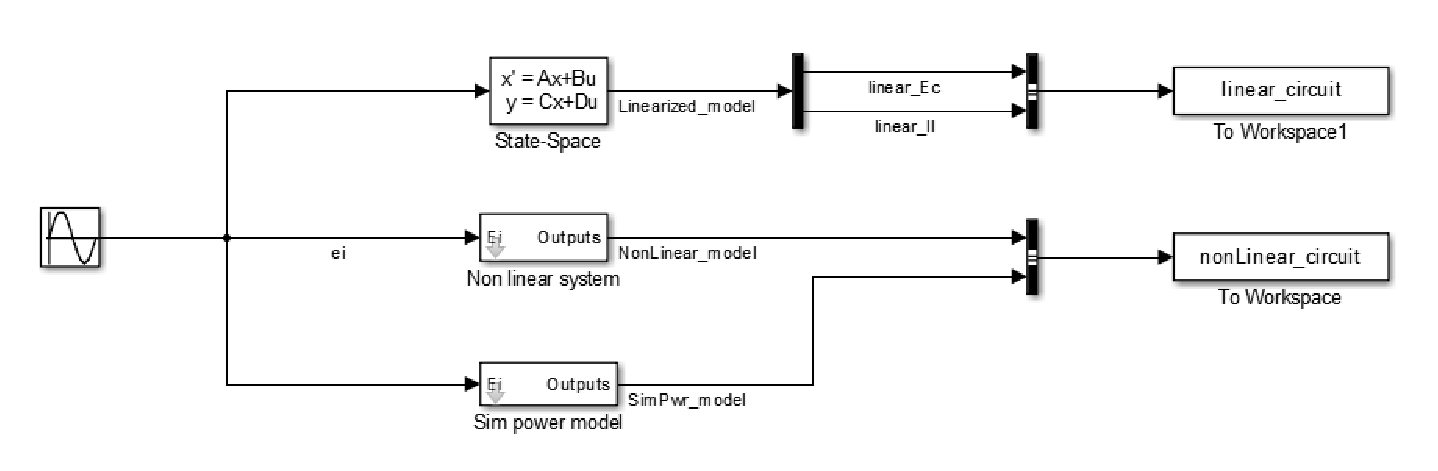
\includegraphics[width=1\textwidth]{Ex1_Simulink.eps}
	\caption{Simulink model used for electrical simulation and comparison}
\end{figure}

Ce type de montage permet de vérifier qu'en tout temps la sortie du modèle représenté par le système d'équations non linéaires est égale à la sortie générée par le modèle de type SimPower.
Le modèle ici étant très simple, il n'est pas nécessaire d'ajouter une tolérance sur l'assertion.

\newpage
Dans un soucis de clareté, des sous-systèmes sont utilisés:

\begin{figure}
  \centering      
    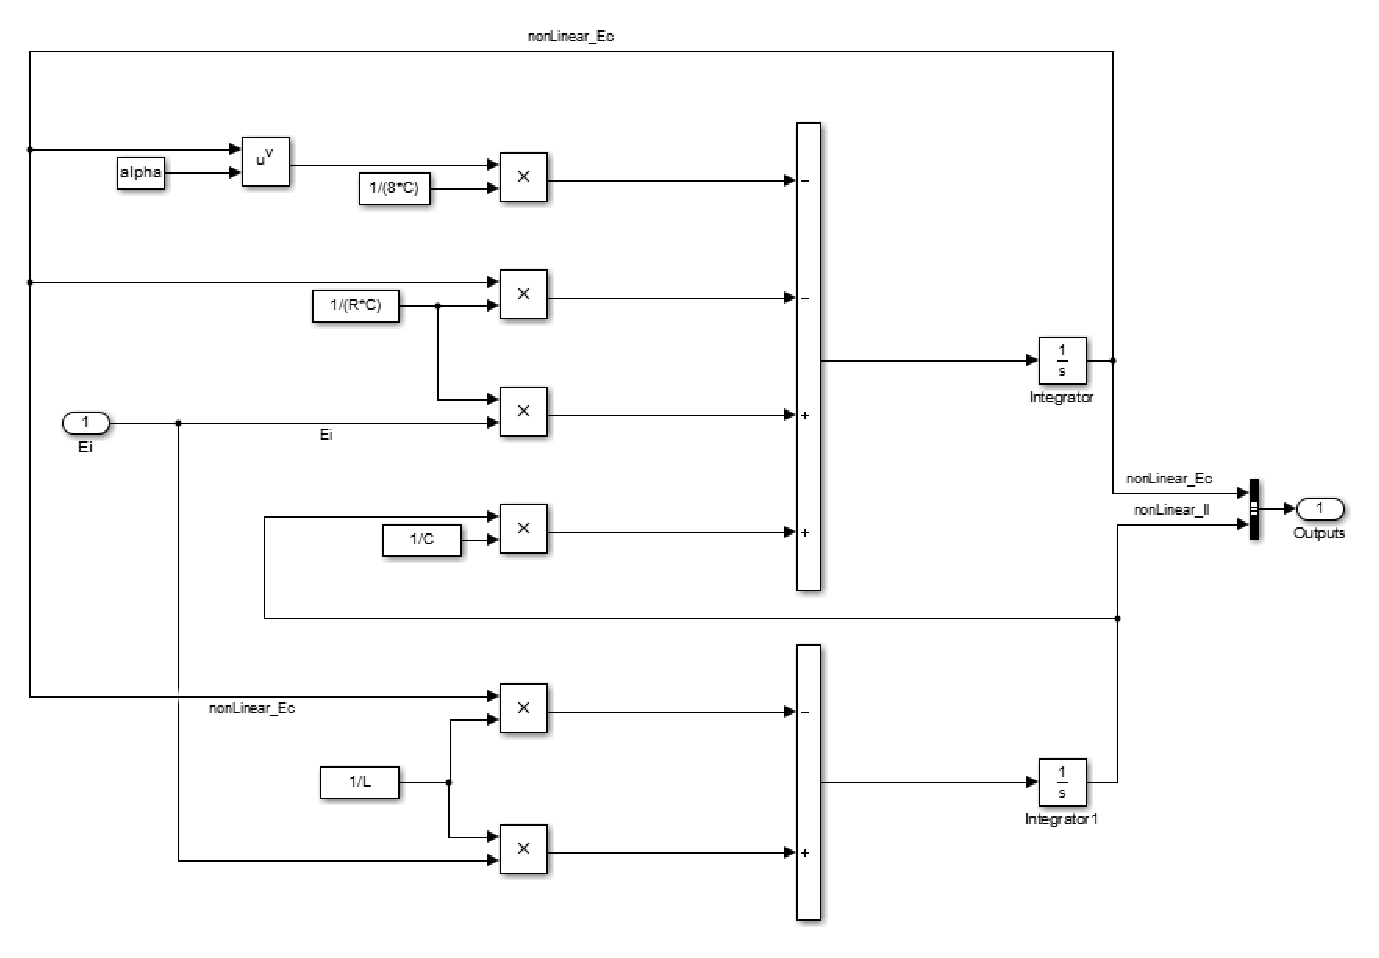
\includegraphics[width=1\textwidth]{Ex1_ExactModel.eps}
	\caption{Simulink exact model}
\end{figure}

\begin{figure}
  \centering      
    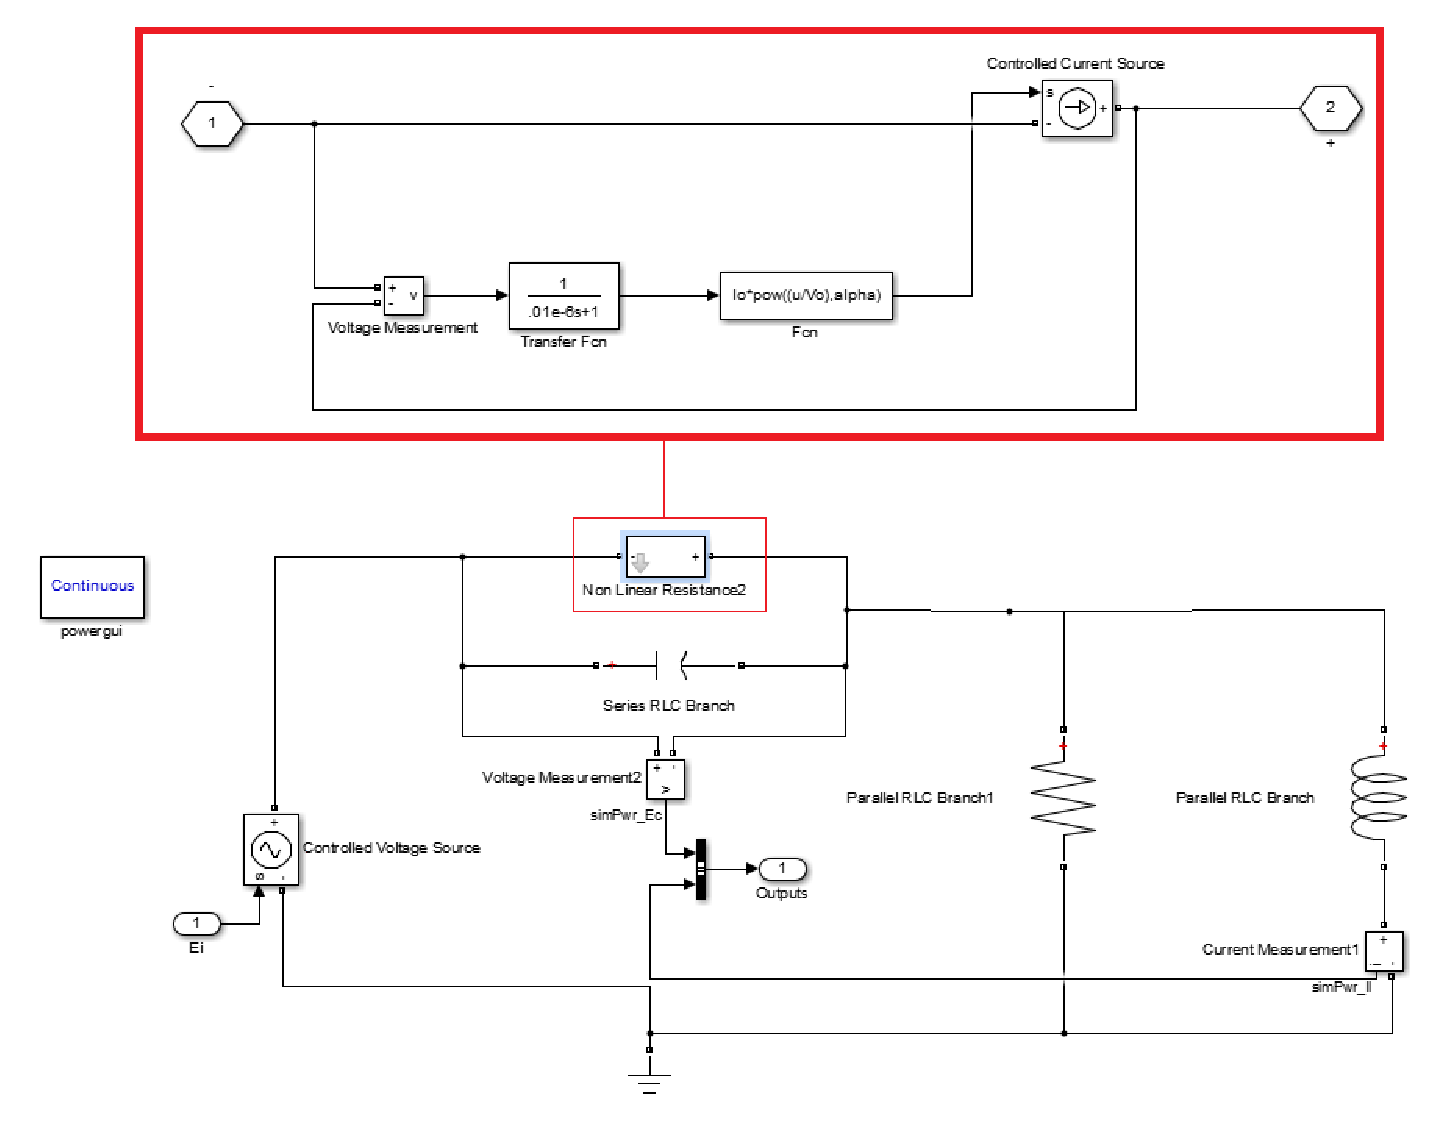
\includegraphics[width=1\textwidth]{Ex1_SimPower.eps}
	\caption{Simpower model}
\end{figure}

\begin{figure}
  \centering      
    \includegraphics[width=1\textwidth]{Ex1_StateSpace.eps}
	\caption{Simpower linearized state space model}
\end{figure}

\FloatBarrier
 \pagebreak[4]
\item \underline{Résultats}

On trace et on superpose, pour trois valeurs différentes d'amplitude de la source de tension, l'intensité aux bornes de la bobine.
Avec une amplitude très faible, la bobine est presque équivalente à un court circuit tandis que le condensateur équivaut à une borne ouverte. 
Le circuit est alors équivalent à la seule résistance non linéaire en série avec la source de tension, la tension a ses bornes est équivalente à la tension aux bornes de la source, en conséquence l'intensitée attendue aux bornes de l'inducteur est $-\frac{1}{8C}\Vc^3 = 1A$.
L'annulation des états dérivés du circuit doit donc se matérialiser par un circuit pratiquement linéaire. Ceci est confirmé sur les courbes suivantes:

%Figure matlbal exo1
\begin{figure}
  \centering      
    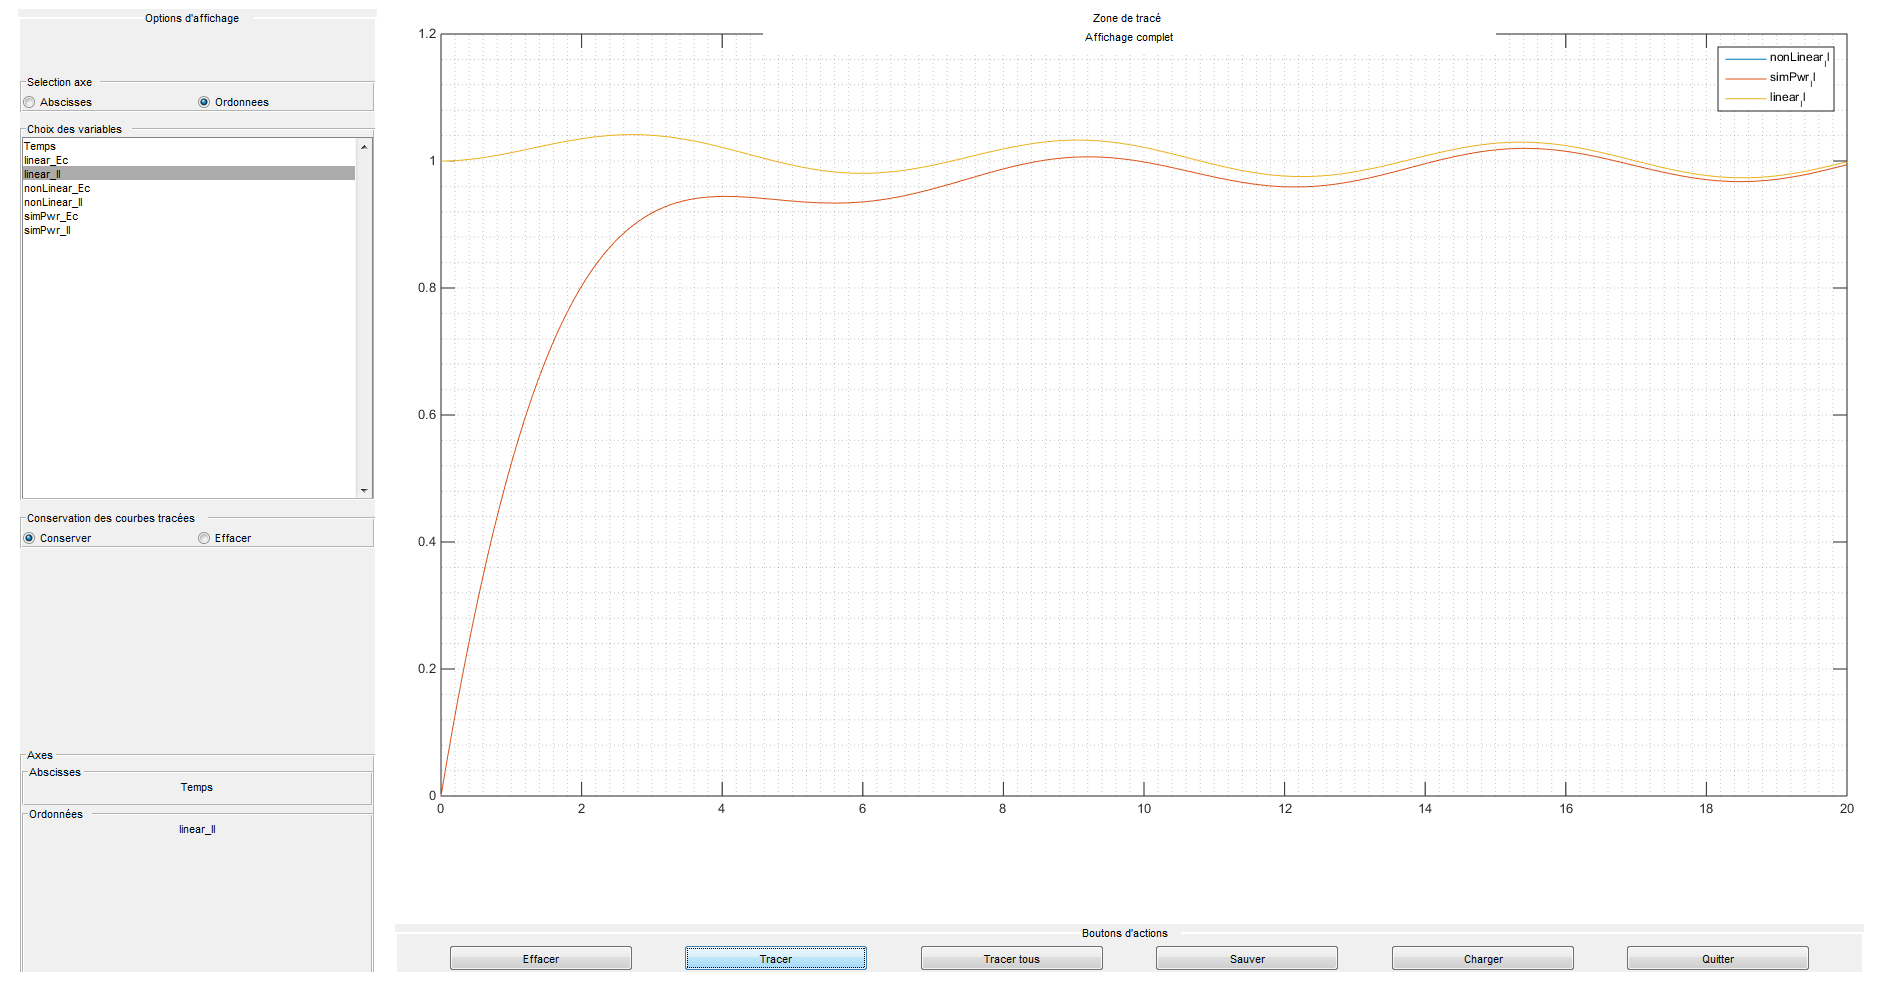
\includegraphics[angle=90, scale=.4, keepaspectratio=true]{Ex1_0dec1_Il.eps}
	\caption{Courbe d'intensité au cours du temps avec A=0.1V}
\end{figure}

\begin{figure}
  \centering   
    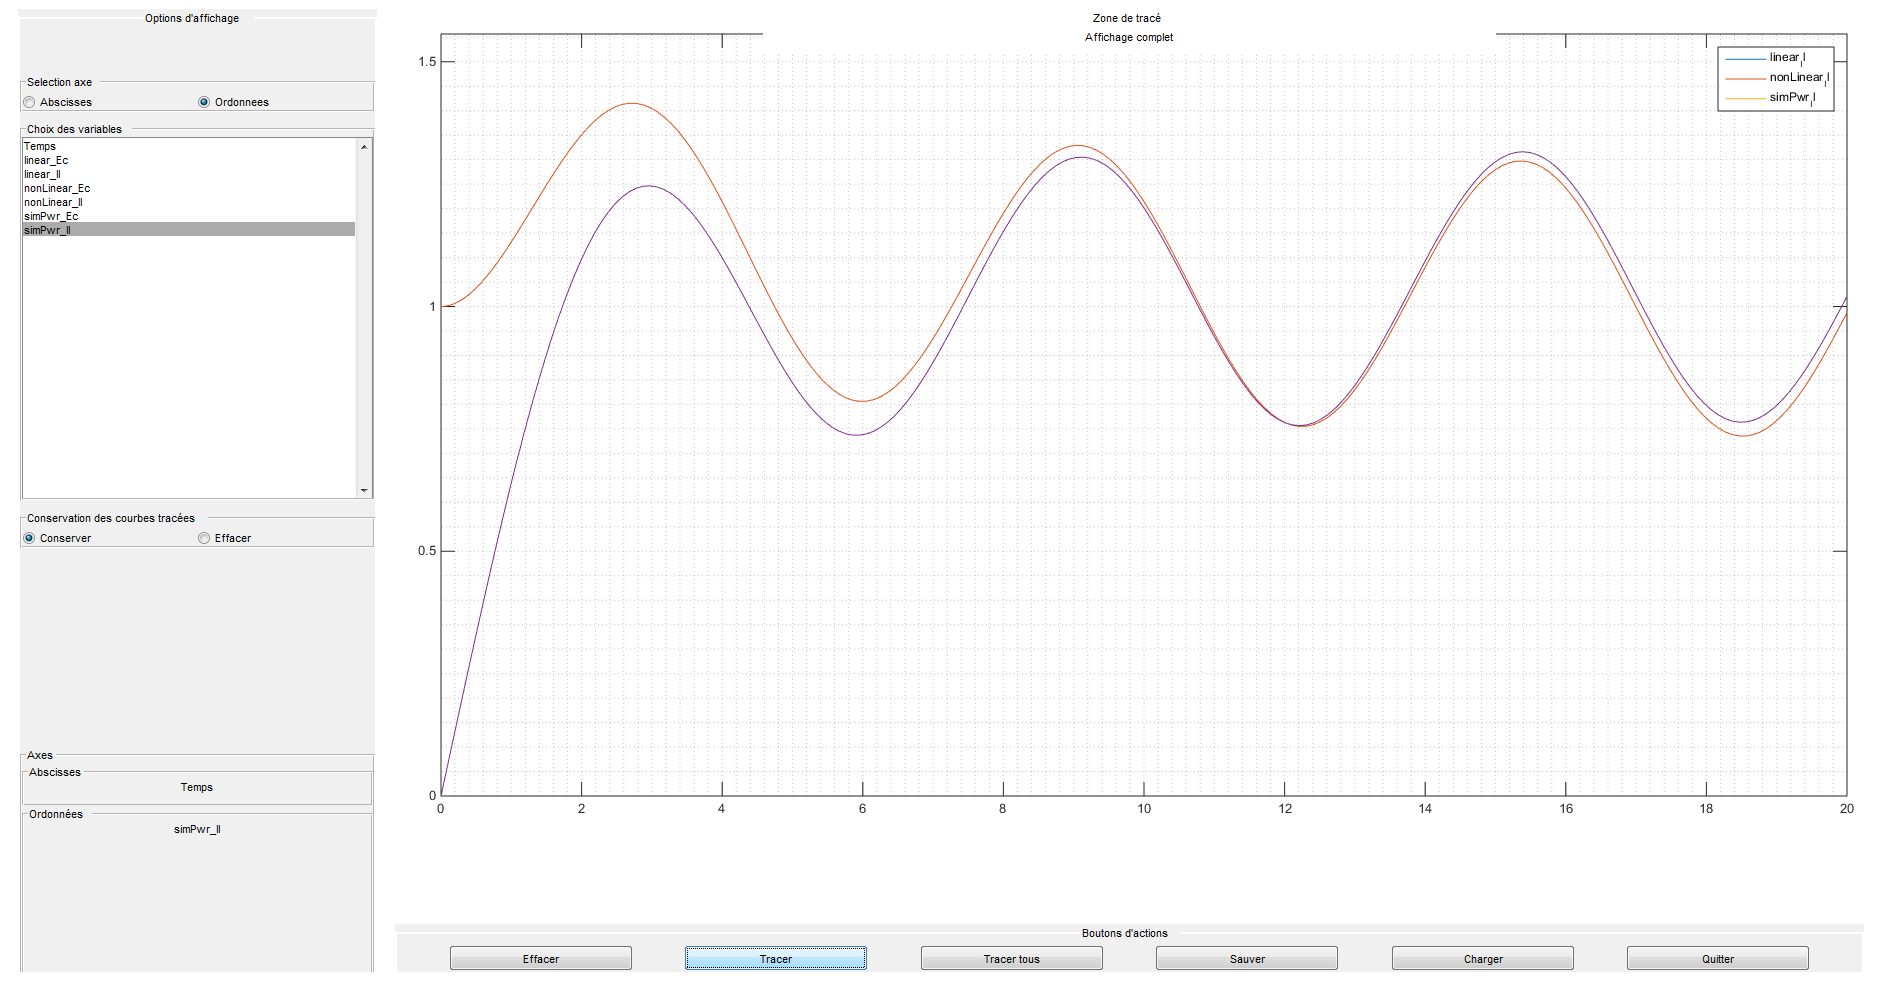
\includegraphics[angle=90, scale=.4, keepaspectratio=true]{Ex1_1_Il.eps}
	\caption{Courbe d'intensité au cours du temps avec A=1V}
\end{figure}

\begin{figure}
  \centering   
    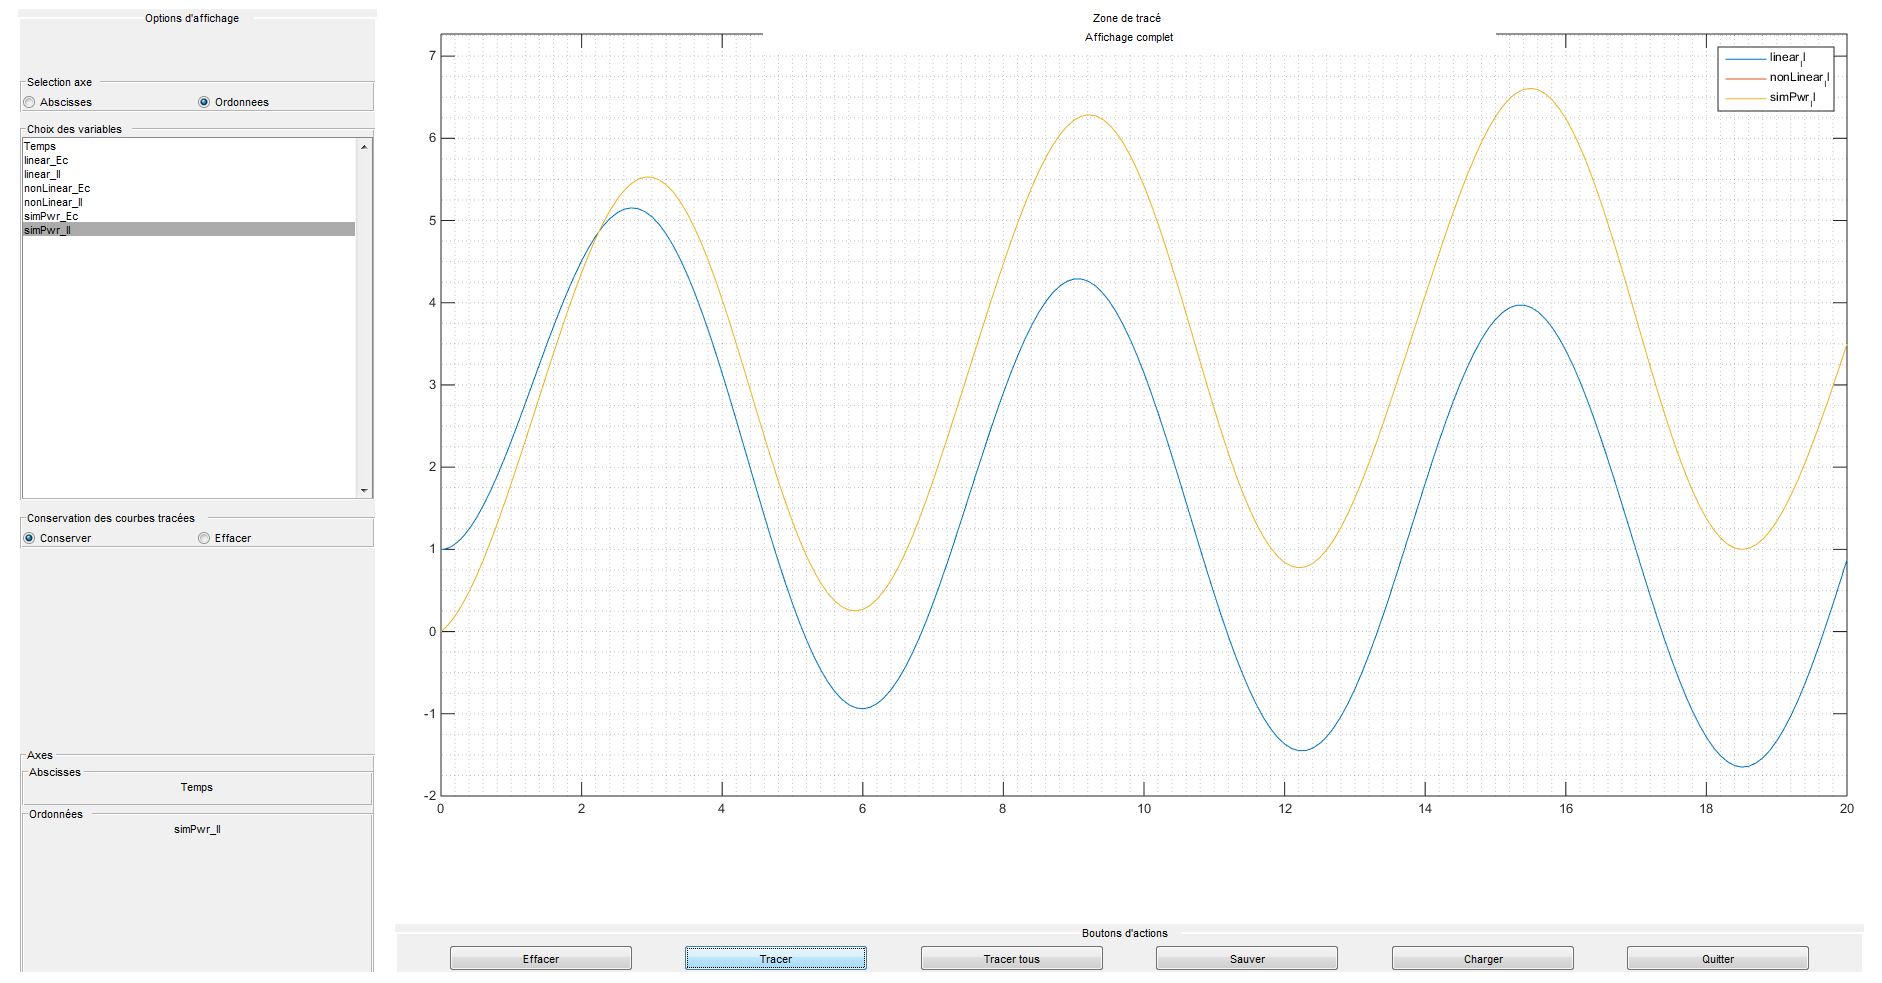
\includegraphics[angle=90, scale=.4, keepaspectratio=true]{Ex1_10_Il.eps}
	\caption{Courbe d'intensité au cours du temps avec A=10V}
\end{figure}

\FloatBarrier
\newpage
Ces courbes permettent de tirer les deux conclusions suivantes:

\begin{itemize}
  \item Le modèle linéarisé ne permet pas de représenter les modes transitoires.\\ Ceci est normal puisque le modèle linéaire n'est représentatif qu'autour de l'équilibre.\\ Les valeurs initiales sont donc faussées.
  \item Le modèle linéarisé offre une plage de résultats relativement acceptables jusqu'à $A=1A$.\\ Au dela les valeurs n'ont aucune représentativité au regard de la part alternative de la source de tension.
\end{itemize}
\end{enumerate}

% START OF EXERCICE 2 %
\newpage
\section{\textbf{Problème 2}}
Système masse ressort non linéaire
\begin{enumerate}
\item \underline{Écrire les équations différentielles qui modélisent ce système.}

Il est admis que la masse est située à $\Xzero$ à l'état d'équilibre.
Par suite, l'équation d'équilibre s'écrit:

\begin{equation*}\label{eq:Ex2:1}
-\M.g+\Kone.(\Xl-\Xzero) = 0
\end{equation*}

Il en résulte l'élongation naturelle du ressort:

\begin{equation}\label{eq::Ex2:2}
\boxed{\Xl = \XlLit}
\end{equation}

En ignorant le plateau amortisseur, on établit l'équation libre du mouvement:

\begin{align}\label{eq::Ex2:3}
\M.\ddX =& -\M.g-\Kone(\X-\Xl) \nonumber \\
\ddX =& -g-\frac{\Kone}{\M}(\X-\Xl) \nonumber \\
\ddX =& -g-\frac{\Kone}{\M}(\X-(\XlLit))
\end{align}

Lorsque le plateau amortisseur est compressé, l'équation devient:

\begin{align}\label{eq::Ex2:4}
\ddX =& -g-\frac{\Kone}{\M}(\X-\Xl)-\frac{\Ktwo}{\M}(\X-\Xone)-\frac{\B}{\M}\dX
\end{align}

Cependant, il convient de noter qu'en l'absence de viscosité le plateau ne peut exercer qu'une action positive sur la masse aussi l'hypothèse suivante est effectuée:

\textit{
La masse remontant plus vite que le plateau en raison de l'action du ressort $\Kone$, l'action du plateau n'est pas constante lorsque $\dX > 0$. Or la masse du plateau amortisseur étant considérée comme nulle on obtient:
\begin{center}
$\lim_{Mp_ \to 0} -\frac{\Ktwo}{Mp}(\X-\Xone)-\frac{\B}{Mp}\dX = \frac{d^2Xp}{dt^2} = \infty$
\end{center}
On considère donc le plateau en contact constant durant la phase de remontée.}

Il en résulte l'équation finale:
\begin{align*}\label{eq::Ex2:5}
\ddX =& -g-\frac{\Kone}{\M}(\X-(\XlLit))+f(\X)
\end{align*}
\begin{empheq}[left=\empheqlbrace]{align*}
f(\X) &= 0 ,\ \X >= \Xone\\
f(\X) &= \min[-\frac{\Ktwo}{\M}(\X-\Xone)-\frac{\B}{\M}\dX,0] ,\ \X < \Xone
\end{empheq}

Pour la suite de l'exercice on note:

\begin{align}\label{eq::Ex2:6}
\Aboxed{\ddX =& \Fm(\X) + \Fs(\X)}
\end{align}

\begin{empheq}[left=\empheqlbrace, box=\fbox]{align}
\Fm(\X) &= -g-\frac{\Kone}{\M}(\X-(\XlLit)) &,\forall \X \nonumber \\
\Fs(\X) &= 0 &,\X >= \nonumber \Xone\\
\Fs(\X) &= \min[-\frac{\Ktwo}{\M}(\X-\Xone)-\frac{\B}{\M}\dX,0] &,\X < \Xone
\end{empheq}


\item \underline{Simuler le système.}

Pour modéliser la non linéarité, nous utilisons dans un cas un bloc switch, dans un autre cas un bloc matlab function représentant le bloc switch.
Le modèle est par soucis de clarté décomposé en deux sous-systèmes, l'un représentant $\Fm(\X)$ et l'autre $\Fs(\X)$.
Note: afin de valider le modèle, un frottement visqueux est rajouté à $\Fm(\X)$. Compte tenu des vitesses mises en jeu, un frottement de type $f(v)$ au lieu de $f(v^2)$ est acceptable.
Cet amortissement est nul durant les simulations présentées dans ce rapport.

\begin{figure}
  \centering      
    \includegraphics[width=1\textwidth]{Ex2_Simulink.eps}
	\caption{Simulink overview}
	\label{Ex:Simulink:1}
\end{figure}

\begin{figure}
  \centering      
    \includegraphics[width=1\textwidth]{Ex2_Simulink_Fm.eps}
	\caption{Fm}
	\label{Ex:Simulink:2}
\end{figure}

\begin{figure}
  \centering      
    \includegraphics[width=1\textwidth]{Ex2_Simulink_Fs.eps}
	\caption{Fs}
	\label{Ex:Simulink:3}
\end{figure}

\FloatBarrier
 \pagebreak[4]
 
\item \underline{Présentation des résultats.}

On trace les courbes associées à $\X, \Fs(\X)$ et $\dX$ pour $K_2=1, b=1$:

\begin{figure}
  \centering      
    \includegraphics[angle=90, scale=.4, keepaspectratio=true]{Ex2_Simu1_k1_b1.eps}
	\caption{Évolutions de $\X, \Fs(\X)$ et $\dX$ pour $K_2=1, b=1$}
	\label{Ex:Resultats:1}
\end{figure}

La figure \ref{Ex:Resultats:1} permet de voir que la force $F_s$ ne s'applique que pour $x<1$ et est strictement positive.

On trace ensuite le déplacement maximal de la masse en fonction de $K_2$ et $b$. Pour une meilleure résolution le pas de valeur est de 1 entre 10 et 50 pour chacune des variables.

\begin{figure}
  \centering      
    \includegraphics[angle=90, scale=.4, keepaspectratio=true]{Ex2_DepMax.eps}
	\caption{Déplacement maximal de la masse depuis sa position d'origine.}
	\label{Ex:Resultats:2}
\end{figure}

Il apparait clairement que le déplacement minimal est atteint aux valeurs maximales de $K_2$ et $b$.
Cependant pour des raisons de coût et d'optimisation, il est pertinent de s'intéresser au gain procuré par les plus faibles valeurs de $K_2$ et $b$. 
La figure \ref{Ex:Resultats:2} montre clairement que le gain est très fort lorsque $K_2$ et $b$ augmentent faiblement alors que leurs valeurs sont elles même faibles. Mais ce gain diminue rapidement.

On s'intéresse donc au lieu des gradients tels que $\vec\nabla(X_{Min}(k2,b)) < 0.01$. Cette valeur est arbitraire et on la considère comme étant le seuil à partir duquel le gain est nul.

\begin{figure}
  \centering      
    \includegraphics[width=1\textwidth]{Ex2_LieuxGrad.eps}
	\caption{Lieux des gradients}
	\label{Ex:Resultats:3}
\end{figure}

\FloatBarrier

La figure \ref{Ex:Resultats:3} montre qu'il est possible de choisir le couple $(K_2,b)$ dans des plages de valeurs acceptables telles que (25,20).
En comparaison, le gain avec le couple (50,50) n'est que de $6\%$.
Cette façon de faire laisse également plus de choix pour répondre aux contraintes de confort, ou d'effort applicable à la masse, tout en gardant un amortissement équivalent.

\end{enumerate}

 \pagebreak[4]
\begin{center}
\section*{\textbf{ANNEXES: Code Matlab}}
\end{center}

\begin{enumerate}
\item \underline{Exercice1 : Code d'exécution}

\lstinputlisting{circuitElectriqueDataDictionnary.m}

\newpage
\item \underline{Exercice1 : Code de post-process}

\lstinputlisting{circuitElectriquePost.m}

\newpage
\item \underline{Exercice2 : Code d'exécution}

\lstinputlisting{masseRessortDataDictionnary.m}

\newpage
\item \underline{Exercice2 : Code de post-process}

\lstinputlisting{masseRessortDataPost.m}

\newpage
\item \underline{Exercice2 : Code du bloc switch}

\begin{lstlisting}
function Fs = fcn(u,cond)
%#codegen

if (cond > 0)
    Fs = u;
else
    Fs = 0;
end
\end{lstlisting}
\end{enumerate}


\begin{center}
\vspace{3cm}
--------- \textit{\lastwords} ---------
\end{center}


\label{finalpage}

\end{document}
